\documentclass[aspectratio=169,usenames,dvipsnames]{beamer}

\usepackage{amsmath}
\usepackage{booktabs}
\usepackage{xcolor}
\usepackage[english]{babel}
\usepackage{unicode-math}
\usepackage{mathtools}
\usepackage{derivative}
\usepackage{makecell}
\usepackage{multirow}
\usepackage{siunitx}
\usepackage{pgfplots}
\usepackage{circuitikz}
\usepackage{appendixnumberbeamer}

\usetheme{metropolis}

\setmainfont{Stix Two Text}
\setmathfont{Stix Two Math}

\input{math}

\pgfplotsset{compat=1.17}
\usetikzlibrary{arrows.meta}
\usetikzlibrary{fit}
\usetikzlibrary{positioning}
\usepgfplotslibrary{groupplots}

\definecolor{exotic orange}{RGB}{255,128,0}
\definecolor{exotic green}{RGB}{0,102,102}
\definecolor{exotic blue}{RGB}{67,132,161}
\definecolor{exotic red}{RGB}{250,86,86}

\DeclareSIUnit{\arbitraryunit}{arb. unit}

\title{A theoretical framework for CV-QKD}
\date{\today}
\author{Bodo Kaiser}
\institute{Ludwig-Maximilians-Universität München}

\begin{document}
	\maketitle
	
	% why is QKD interesting? -> intersection of multiple disciplines (quantum information theory, quantum optics, communication engineering)	
	\begin{frame}{Preview}
		\begin{columns}[c, onlytextwidth]
			\column{0.6\textwidth}
			\begin{figure}
				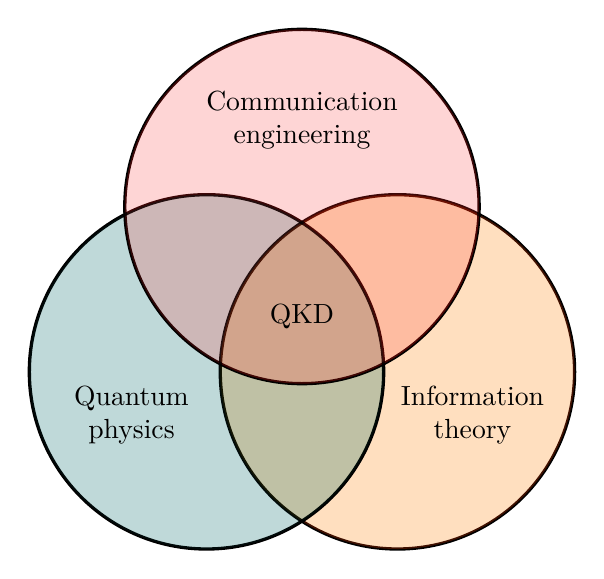
\begin{tikzpicture}[
					venn circle/.style={draw, very thick, fill opacity=0.25, circle, minimum width=45mm},
					venn label/.style={align=center},
				]
					\begin{scope}[blend group=soft light]
						\node[venn circle, fill=exotic red] (qp) at (90:1.4) {};
						\node[venn circle, fill=exotic green] (it) at (210:1.4) {};
						\node[venn circle, fill=exotic orange] (qp) at (330:1.4) {};
					\end{scope}
					
					\node[venn label] {QKD};
					\node[venn label] at (90:2.5) {Communication\\engineering};
					\node[venn label] at (210:2.5) {Quantum\\physics};
					\node[venn label] at (330:2.5) {Information\\theory};
				\end{tikzpicture}
			\end{figure}

			\column{0.4\textwidth}
			\setbeamertemplate{section in toc}[sections numbered]
			\tableofcontents[hideallsubsections]
		\end{columns}
	\end{frame}
	
	\section{Introduction}

	% what is secure communication: integrity and confidentiality	
	% key distribution problem
	% public-key distribution
	% information-theoretical secure for OTP but practically one uses AES
	\begin{frame}{Secure transmission system}
		\begin{figure}
			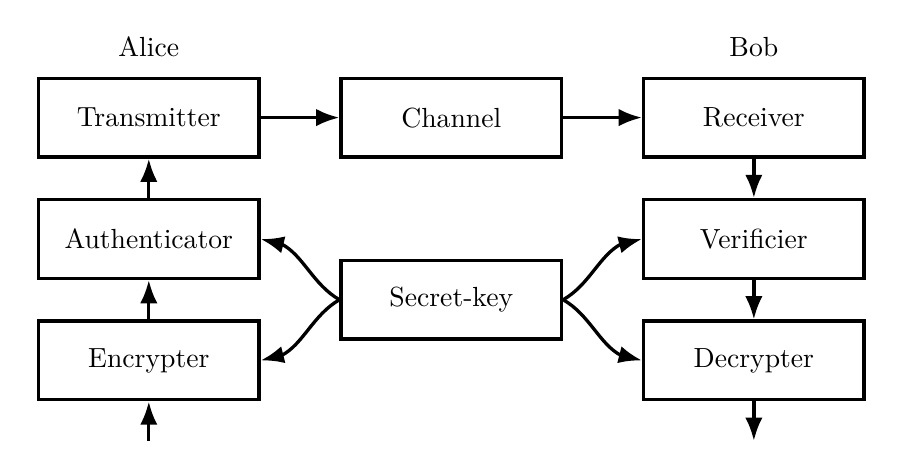
\begin{tikzpicture}[
				node distance=5mm,
				arrow/.style={very thick, -Latex},
				block/.style={draw, very thick, minimum width=28mm, minimum height=10mm},		
			]
				\coordinate (in);
				\node[block, above=of in] (encryption) {Encrypter};
				\node[block, above=of encryption] (authentication) {Authenticator};
				\node[block, above=of authentication] (transmitter) {Transmitter};
				\node[block, right=10mm of transmitter] (channel) {Channel};
				\node[block, right=10mm of channel] (receiver) {Receiver};
				\node[block, below=of receiver] (verification) {Verificier};
				\node[block, below=of verification] (decryption) {Decrypter};
				\coordinate[below=of decryption] (out);
	
				\path (encryption) -- (verification) node[midway, block, align=center] (key) {Secret-key};
	
				\draw[arrow] (key.west) to[out=210, in=0] (encryption.east);
				\draw[arrow] (key.west) to[out=150, in=0]  (authentication.east);
				\draw[arrow] (key.east) to[out=-30, in=180] (decryption.west);
				\draw[arrow] (key.east) to[out=30, in=180] (verification.west);

				\draw[arrow] (in) -- (encryption);
				\draw[arrow] (encryption) -- (authentication);
				\draw[arrow] (authentication) -- (transmitter);
				
				\draw[arrow] (decryption) -- (out);
				\draw[arrow] (verification) -- (decryption);
				\draw[arrow] (receiver) -- (verification);
		
				\draw[arrow] (transmitter) -- (channel.west);
				\draw[arrow] (channel.east) -- (receiver);
				
				\node[label={Alice}, fit=(encryption) (transmitter)] {};
				\node[label={Bob}, fit=(decryption) (receiver)] {};
			\end{tikzpicture}
			\caption{Block diagram of a secure transmission system.}
		\end{figure}
	\end{frame}

    % quantum transmission (random seed, correlated data)
	% post-processing (shared secret key from correlated data)
	\begin{frame}{Quantum key distribution system}
		\begin{figure}
			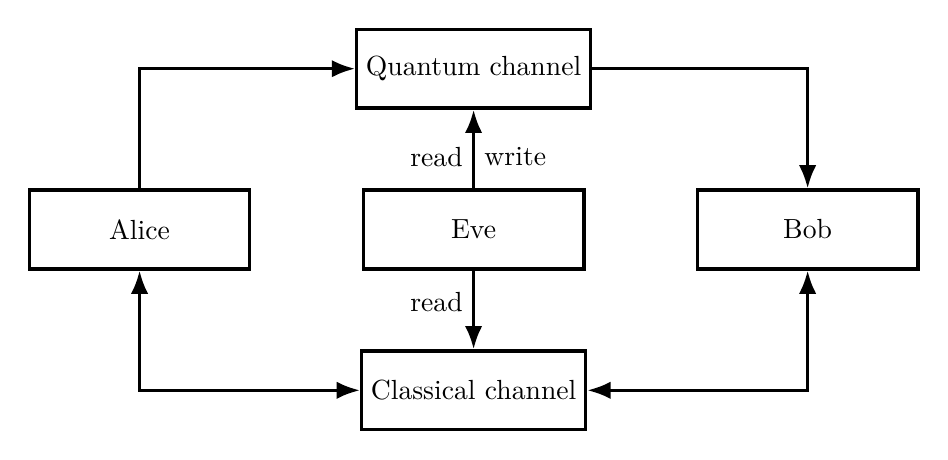
\begin{tikzpicture}[
				node distance=5mm,
				arrow/.style={very thick, -Latex},
				block/.style={draw, very thick, minimum width=28mm, minimum height=10mm},
			]
				\node[block] (alice) {Alice};
				\node[block, right=14mm of alice] (eve) {Eve};
				\node[block, above=10mm of eve] (quantum channel) {Quantum channel};
				\node[block, below=10mm of eve] (classical channel) {Classical channel};
				\node[block, right=14mm of eve] (bob) {Bob};

				\draw[arrow] (eve) -- (classical channel) node[midway, left, yshift=1mm] {read};
				\draw[arrow] (eve) -- (quantum channel) node[midway, left, yshift=-1mm] {read} node[midway, right, yshift=-1mm] {write};
				\draw[arrow] (alice.north) -- (alice.north|-quantum channel.west) -- (quantum channel.west);
				\draw[arrow, Latex-Latex] (alice.south) -- (alice.south|-classical channel.west) -- (classical channel.west);
				\draw[arrow] (quantum channel.east) -- (quantum channel.east-|bob.north) -- (bob.north);
				\draw[arrow, Latex-Latex] (classical channel.east) -- (classical channel.east-|bob.south) -- (bob.south);
			\end{tikzpicture}
			\caption{Block diagram of a quantum key distribution (QKD) system.}
		\end{figure}
	\end{frame}
	
	\begin{frame}{Discrete and continuous-variable QKD}
		\begin{table}[htb]
			\caption{Comparison of discrete- and continuous-variable QKD.}
			\begin{tabular}{lcc}
				\toprule
					& Discrete & Continuous \\
				\midrule
					Visualization & Bloch sphere & Phase space \\
					Hilbert space (dim) & Finite (two) & Countable (infinite) \\
					Observable & $\vb{\hat{S}}(\vb{n})=\hat{S}_in^i$ & $\hat{X}(\vartheta)=\frac{1}{\sqrt{2}}\left(\hat{a}e^{-i\vartheta}+\hat{a}^\dagger e^{+i\vartheta}\right)$ \\
					Standard basis & $\left\{\ket{0},\ket{1}\right\}$ & $\left\{\ket{x},\ket{p}\right\}_{x,p\in\mathbb{R}}$ \\
				\bottomrule
			\end{tabular}
		\end{table}
	\end{frame}
	
	\begin{frame}{Continuous-variable QKD using coherent states}
		\begin{figure}
			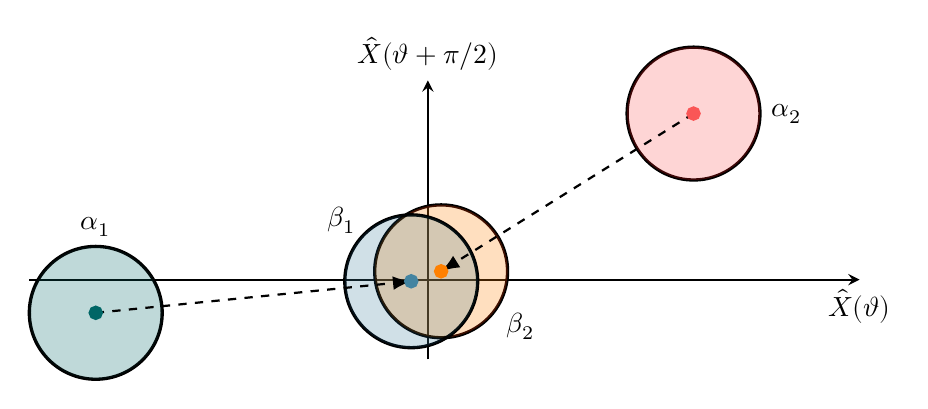
\begin{tikzpicture}[
				var/.style={draw, very thick, fill opacity=0.25, circle, minimum width=45mm},
			]
				\begin{axis}[
					height=6cm,
					width=\linewidth,
					clip=false,
					axis lines=center,
					axis equal image,
					axis line style=thick,
					xlabel={$\hat{X}(\vartheta)$},
					ylabel={$\hat{X}(\vartheta+\pi/2)$},
					ticks=none,
					xmin=-6,
					xmax=+6.5,
					ymin=-1.2,
					ymax=+3,
					axis line style={thick},
					x label style={anchor=north},
					y label style={anchor=south},
				]
					\begin{scope}[blend group=soft light]					
						\draw[var, fill=exotic green] (axis cs:-5,-0.5) circle (1);
						\draw[var, fill=exotic red] (axis cs:4,2.5) circle (1);
						
						\draw[var, fill=exotic blue] (axis cs:-0.25,-0.025) circle (1);
						\draw[var, fill=exotic orange] (axis cs:0.2,0.125) circle (1);
					\end{scope}

					\addplot[very thick, mark=*, exotic green] coordinates {(-5,-0.5)};
					\addplot[very thick, mark=*, exotic red] coordinates {(4,2.5)};					
					\addplot[very thick, mark=*, exotic blue] coordinates {(-0.25,-0.025)};
					\addplot[very thick, mark=*, exotic orange] coordinates {(0.2,0.125)};
					
					\node at (axis cs:-5,0.8) {$\ket{\alpha_1}$};
					\node at (axis cs:5.4,2.5) {$\ket{\alpha_2}$};
					\node at (axis cs:-1.3,0.9) {$\ket{\beta_1}$};
					\node at (axis cs:1.4,-0.7) {$\ket{\beta_2}$};
		
					\draw[-Latex, dashed, thick] (axis cs:-5,-0.5) -- (axis cs:-0.25,-0.025);
					\draw[-Latex, dashed, thick] (axis cs:4,2.5) -- (axis cs:0.2,0.125);
				\end{axis}
			\end{tikzpicture}
			\caption{Phase space diagram of transmitted and received coherent states with mean (dots) and variances (opaque circles).}
		\end{figure}
	\end{frame}
	
	\begin{frame}{Continuous-variable QKD using continuous-time coherent states}
		\begin{figure}
			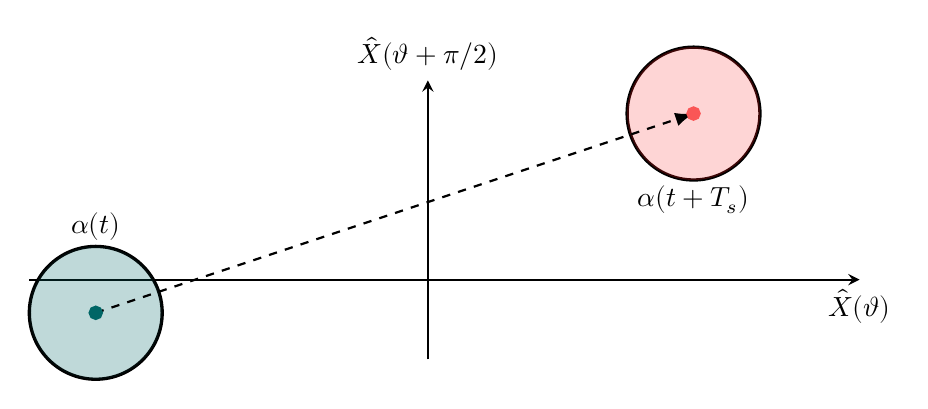
\begin{tikzpicture}[
				var/.style={draw, very thick, fill opacity=0.25, circle, minimum width=45mm},
			]
				\begin{axis}[
					height=6cm,
					width=\linewidth,
					clip=false,
					axis lines=center,
					axis equal image,
					axis line style=thick,
					xlabel={$\hat{X}(\vartheta)$},
					ylabel={$\hat{X}(\vartheta+\pi/2)$},
					ticks=none,
					xmin=-6,
					xmax=+6.5,
					ymin=-1.2,
					ymax=+3,
					axis line style={thick},
					x label style={anchor=north},
					y label style={anchor=south},
				]
					\begin{scope}[blend group=soft light]					
						\draw[var, fill=exotic green] (axis cs:-5,-0.5) circle (1);
						\draw[var, fill=exotic red] (axis cs:4,2.5) circle (1);
					\end{scope}

					\addplot[very thick, mark=*, exotic green] coordinates {(-5,-0.5)};
					\addplot[very thick, mark=*, exotic red] coordinates {(4,2.5)};
					
					\node at (axis cs:-5,0.8) {$\ket{\alpha(t)}$};
					\node at (axis cs:4,1.2) {$\ket{\alpha(t+T_s)}$};
					\draw[-Latex, dashed, thick] (axis cs:-5,-0.5) -- (axis cs:4,2.5);
				\end{axis}
			\end{tikzpicture}
			\caption{Phase space diagram of continuous-time coherent states with mean (dots) and variances (opaque circles) at two time instances.}
		\end{figure}
	\end{frame}
	
	\section{Coherent state transmitter}
	
	\begin{frame}{Software-defined transmitter architecture}
		\begin{figure}
			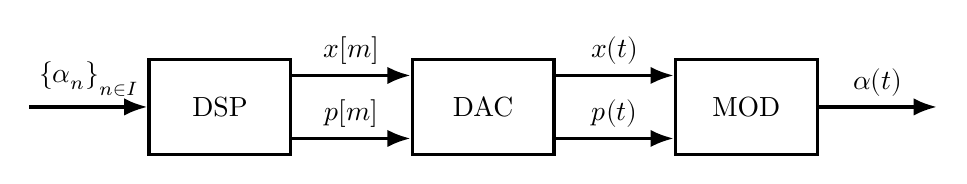
\begin{tikzpicture}[
				node distance=15mm,
				arrow/.style={very thick, -Latex},
				block/.style={draw, very thick, minimum width=18mm, minimum height=12mm},
			]
				\coordinate (in) at (0,0);
				\node (dsp) [block, right=of in] {DSP};
				\node (dac) [block, right=of dsp] {DAC};
				\node (mod) [block, right=of dac] {MOD};
				\coordinate[right=of mod] (out);
				
				\draw[arrow] (in) -- (dsp) node[midway, above] {$\left\{\alpha_n\right\}_{n\in I}$};
				\draw[arrow] ([yshift=4mm]dsp.east) -- ([yshift=4mm]dac.west) node[midway, above] {$x[m]$};
				\draw[arrow] ([yshift=-4mm]dsp.east) -- ([yshift=-4mm]dac.west) node[midway, above] {$p[m]$};
				\draw[arrow] ([yshift=4mm]dac.east) -- ([yshift=4mm]mod.west) node[midway, above] {$x(t)$};
				\draw[arrow] ([yshift=-4mm]dac.east) -- ([yshift=-4mm]mod.west) node[midway, above] {$p(t)$};
				\draw[arrow] (mod) -- (out) node[midway, above] {$\ket{\alpha(t)}$};
			\end{tikzpicture}
			\caption{Block diagram of the software-defined transmitter architecture.}
		\end{figure}
		
		\begin{figure}
			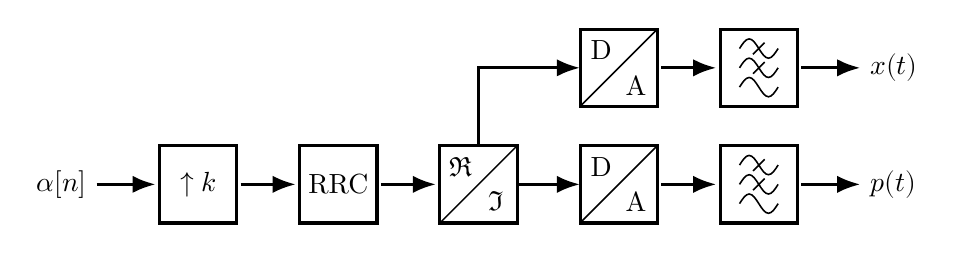
\begin{tikzpicture}[
				line width=0.2mm,
				node distance=8mm,
				arrow/.style={very thick, -Latex},
			]
				\node (in) {$\alpha[n]$};
				\node (up) [twoportshape, right=of in, t={$\uparrow k$}] {};
				\node (rrc) [twoportshape, right=of up, t=RRC] {};
				\node (real) [twoportsplitshape, circuitikz/t1={$\Re$}, circuitikz/t2={$\Im$}, right=of rrc] {};

				\node (dacp) [dacshape, right=of real] {};
				\node (lowp) [lowpassshape, right=of dacp] {};
				\node (outp) [right=of lowp] {$p(t)$};
				
				\node (dacx) [dacshape, above=5mm of dacp] {};
				\node (lowx) [lowpassshape, right=of dacx] {};
				\node (outx) [right=of lowx] {$x(t)$};
				
				\draw[arrow] (in) -- (up);
				\draw[arrow] (up) -- (rrc);
				\draw[arrow] (rrc) -- (real);
		
				\draw[arrow] (real.north) -- (real.north|-dacx.west) -- (dacx.west);
				\draw[arrow] (dacx) -- (lowx);
				\draw[arrow] (lowx) -- (outx);
		
				\draw[arrow] (real.east) -- (real.east|-dacp.west) -- (dacp.west);
				\draw[arrow] (dacp) -- (lowp);
				\draw[arrow] (lowp) -- (outp);
			\end{tikzpicture}
			\caption{Block diagram of the digital signal processing for symbol encoding.}
		\end{figure}
	\end{frame}

	\begin{frame}{Symbol-encoding in the time domain}
		\begin{figure}
			\begin{tikzpicture}
				\begin{groupplot}[
					group style={
						group name=plot,
						group size=2 by 4,
						vertical sep=2mm,
						horizontal sep=26mm,
					},
					xmin=10,
					xmax=20,
					ylabel style={align=center},
					grid=major,
					width=0.44\linewidth,
					height=37mm,
					cycle list name=exotic,
					axis line style={thick},
				]
					\nextgroupplot[
						xticklabels={},
						ylabel={Ampl. $\alpha[km]$\\(\si{\arbitraryunit})},
					]
					\addplot+[
						very thick,
						ycomb,
						mark=o,
						restrict expr to domain={\thisrow{c1}}{10:20},
					] plot table[col sep=comma] {./data/rand-time-tx-sym-real.csv};
					\addplot+[
						very thick,
						ycomb,
						mark=x,
						restrict expr to domain={\thisrow{c1}}{10:20},
					] plot table[col sep=comma] {./data/rand-time-tx-sym-imag.csv};
					\nextgroupplot[
						xticklabels={},
						ylabel={Ampl. $\gamma[m]$\\(\si{\arbitraryunit})},
					]
					\addplot+[
						very thick,
						ycomb,
						mark=o,
						restrict expr to domain={\thisrow{c1}}{10:20},
					] plot table[col sep=comma] {./data/rand-time-tx-rrc-real.csv};
					\addplot+[
						very thick,
						ycomb,
						mark=x,
						restrict expr to domain={\thisrow{c1}}{10:20},
					] plot table[col sep=comma] {./data/rand-time-tx-rrc-imag.csv};
					\nextgroupplot[
						ylabel={Ampl. $\rho[m]$\\(\si{\arbitraryunit})},
						xlabel={Symbol index $km$},
					]
					\addplot+[
						very thick,
						ycomb,
						mark=o,
						restrict expr to domain={\thisrow{c1}}{10:20},
					] plot table[col sep=comma] {./data/rand-time-tx-up-real.csv};
					\addplot+[
						very thick,
						ycomb,
						mark=x,
						restrict expr to domain={\thisrow{c1}}{10:20},
					] plot table[col sep=comma] {./data/rand-time-tx-up-imag.csv};
					\nextgroupplot[
						xlabel={Signal time $t/T_s$},
						ylabel={Ampl. $\alpha(t)$\\(\si{\volt})},
					]
					\addplot+[
						very thick,
						no markers,
						restrict expr to domain={\thisrow{c1}}{10:20},
					] plot table[col sep=comma, y expr=\thisrow{c2}*4] {./data/rand-time-tx-lp-real.csv};
					\addplot+[
						very thick,
						no markers,
						restrict expr to domain={\thisrow{c1}}{10:20},
					] plot table[col sep=comma, y expr=\thisrow{c2}*4] {./data/rand-time-tx-lp-imag.csv};
				\end{groupplot}
			\end{tikzpicture}
			\caption{Symbol-encoding steps in the time domain for random QPSK sequence with real (orange) and imaginary (green) part.}
		\end{figure}
	\end{frame}
	
	\begin{frame}{Symbol-encoding steps in the frequency domain}
		\vspace{-6mm}
		\begin{figure}
			\begin{tikzpicture}
				\begin{groupplot}[
					group style={
						group name=plot,
						group size=2 by 3,
						vertical sep=2mm,
						horizontal sep=26mm,
					},
					grid=major,
					width=0.44\linewidth,
					height=30mm,
					xmin=-4,
					xmax=4,
					xtick distance=1,
					ymin=-60,
					ymax=5,
					ylabel style={align=center},
					axis line style={thick},
					cycle list name=exotic,
				]
					\nextgroupplot[
						xticklabels={},
						ylabel={PSD $\alpha[m]$\\(\si{\decibel})},
					]
					\addplot+[
						very thick,
						no markers,
					] plot table[col sep=comma] {./data/rand-freq-tx-sym.csv};
					\addplot+[
						very thick,
						no markers,
					] plot table[col sep=comma] {./data/unit-freq-tx-sym.csv};
					
					\nextgroupplot[
						xticklabels={},
						ylabel={PSD $\gamma(t)$\\(\si{\decibel})},
					]
					\addplot+[
						very thick,
						no markers,
					] plot table[col sep=comma] {./data/rand-freq-tx-dac.csv};
					\addplot+[
						very thick,
						no markers,
					] plot table[col sep=comma] {./data/unit-freq-tx-dac.csv};

					\nextgroupplot[
						xticklabels={},
						ylabel={PSD $\rho[m]$\\(\si{\decibel})},
					]
					\addplot+[
						very thick,
						no markers,
					] plot table[col sep=comma] {./data/rand-freq-tx-up.csv};
					\addplot+[
						very thick,
						no markers,
					] plot table[col sep=comma] {./data/unit-freq-tx-up.csv};					
					
					\nextgroupplot[
						xlabel={Frequency $f/f_s$},
						ylabel={PSD $\alpha(t)$\\(\si{\decibel})},
					]
					\addplot+[
						very thick,
						no markers,
					] plot table[col sep=comma] {./data/rand-freq-tx-lp.csv};
					\addplot+[
						very thick,
						no markers,
					] plot table[col sep=comma] {./data/unit-freq-tx-lp.csv};
					
					\nextgroupplot[
						xlabel={Frequency $f/f_s$},
						ylabel={PSD $\gamma[m]$\\(\si{\decibel})},
					]
					\addplot+[
						very thick,
						no markers,
					] plot table[col sep=comma] {./data/rand-freq-tx-rrc.csv};
					\addplot+[
						very thick,
						no markers,
					] plot table[col sep=comma] {./data/unit-freq-tx-rrc.csv};
				\end{groupplot}
			\end{tikzpicture}
			\caption{Symbol-encoding steps in the frequency domain for random symbols (green) and single symbol (orange).}
		\end{figure}
	\end{frame}
		
	\begin{frame}{Upconversion}
		
	\end{frame}
	
	\begin{frame}{In-phase and quadrature modulator}
		
	\end{frame}
	
	\section{Coherent state receiver}
	
	\begin{frame}{Software-defined receiver architecture}
		\begin{figure}
			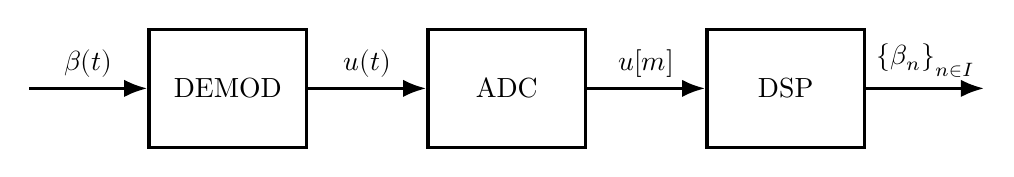
\begin{tikzpicture}[
				node distance=15mm,
				arrow/.style={very thick, -Latex},
				block/.style={draw, very thick, minimum width=20mm, minimum height=15mm},
			]
				\coordinate (in) at (0,0);
				\node (dsp) [block, right=of in] {DEMOD};
				\node (dac) [block, right=of dsp] {ADC};
				\node (mod) [block, right=of dac] {DSP};
				\coordinate[right=of mod] (out);
				
				\draw[arrow] (in) -- (dsp) node[midway, above] {$\ket{\beta(t)}$};
				\draw[arrow] (dsp.east) -- (dac.west) node[midway, above] {$u(t)$};
				\draw[arrow] (dac.east) -- (mod.west) node[midway, above]{$u[m]$};
				\draw[arrow] (mod) -- (out) node[midway, above] {$\left\{\beta_n\right\}_{n\in I}$};
			\end{tikzpicture}
			\caption{Block diagram of software-defined transmitter architecture including symbol encoding in the digital domain, digital-to-analog conversion and electro-optical modulation.}
		\end{figure}
	\end{frame}
	
	\begin{frame}{Downconversion}
		
	\end{frame}
	
	\begin{frame}{Balanced detector}
		
	\end{frame}
	
	\section{Conclusion and outlook}
	
	\begin{frame}{Conclusion and outlook}
	\end{frame}
	
	\appendix
	
	\begin{frame}{Classical post-processing pipeline}
		\begin{figure}
	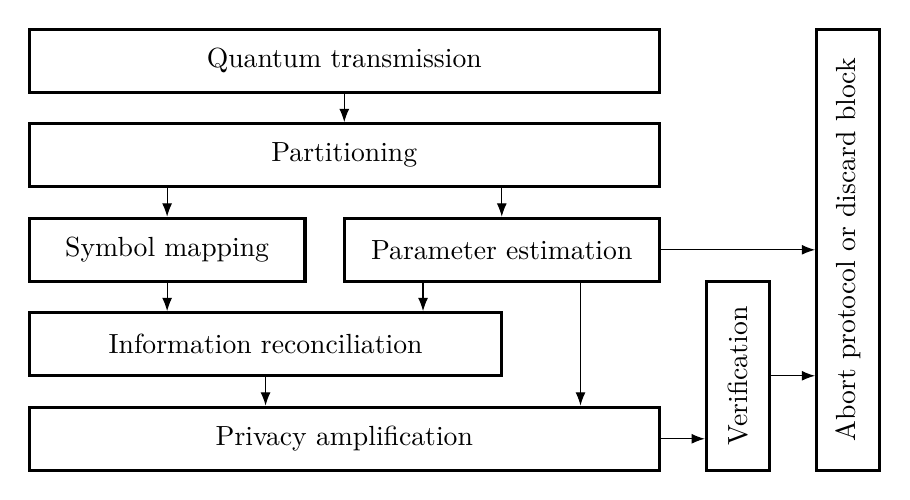
\begin{tikzpicture}[
		block/.style={draw, very thick, minimum height=8mm},
	]
		\node[block, minimum width=8cm] (qt) at (0,0) {Quantum transmission};
		\node[block, minimum width=8cm] (pt) at (0,-1.2) {Partitioning};
		
		\node[block, minimum width=3.5cm] (sm) at (-2.25,-2.4) {Symbol mapping};
		\node[block, minimum width=4cm] (pe) at (2,-2.4) {Parameter estimation};
		\node[block, minimum width=6cm] (ir) at (-1,-3.6) {Information reconciliation};
		\node[block, minimum width=8cm] (pa) at (0,-4.8) {Privacy amplification};

		\draw[-Latex] (qt) -- (pt);
		\draw[Latex-] (sm.north) -- (sm.north|-pt.south);
		\draw[Latex-] (pe.north) -- (pe.north|-pt.south);
		\draw[-Latex] (sm.south) -- (sm.south|-ir.north);
		\draw[-Latex] (ir.south) -- (ir.south|-pa.north);

		\begin{scope}[transform canvas={xshift=-1cm}]
			\draw[-Latex] (pe.south) -- (pe.south|-ir.north);
		\end{scope}
		\begin{scope}[transform canvas={xshift=1cm}]
			\draw[-Latex] (pe.south) -- (pe.south|-pa.north);
		\end{scope}
		
		\node[block, rotate=90, minimum width=2.4cm] (ver) at (5,-4) {Verification};
		\node[block, rotate=90, minimum width=5.6cm] (abort) at (6.4,-2.4) {Abort protocol or discard block};
		\draw[-Latex] (pe.east) -- (pe.east-|abort.north);
		\draw[-Latex] (pa.east) -- (pa.east-|ver.north);
		\draw[-Latex] (ver.south) -- (ver.south-|abort.north);
	\end{tikzpicture}
		\caption{Block diagram of classical post-processing pipeline.}
		\end{figure}
	\end{frame}

\end{document}